% Chapter 1

\chapter{Summative Evaluation} % Main chapter title

\label{summativeevalchapter} % For referencing the chapter elsewhere, use \ref{Chapter1} 

\lhead{Chapter \ref{summativeevalchapter}. \emph{Summative Evaluation}} % This is for the header on each page - perhaps a shortened title

%----------------------------------------------------------------------------------------
\section{Recruitment of Participants}
With help of a research assistant who was a resident of Langa,  we managed to recruit a total of fourteen adult participants (beneficiary users). We recruited these participants from two townships in Cape Town: Langa, and Athlone. In Langa there were six adult participants while in Athlone there were nine adult participants. The average age of these adult participants was 44.21 years with a standard deviation (S.D) of 9.99 years. The youngest adult was 26 years of age while the oldest was 60 years of age. Thirteen participants were females. 

Each adult participant (beneficiary user) elected one of their children/grand children to become their intermediary user to form a pair of users. The two members of a pair were required to work together in using the ``Family Wellness App'' to self-monitor the wellness of one member of a pair (a beneficiary user). All beneficiary users were working with their children but one whom was was working with her grand child.  The average age of children participants (intermediary users) was 15.42 (S.D=2.06) years. The youngest intermediary user was 12 years of age while the oldest was 20 years of age. The number of females and males intermediary users were equal. 

I gave detailed information of what the study was all about to both intermediary and beneficiary participants. I informed them about different modes of which I will collect data. All beneficiary participants signed informed consent forms agreeing to be part of the study. Since all intermediaries were under 21 years of age, they signed assent forms which were also signed by their parents/guardians who were part of the study.

I allocated one day to teach intermediary participants on how to use the ``Family Wellness App''. In addition, each intermediary was given a user manual. After the training, I gave out one Android phone (Samsung GT-S5300) to each pair of participants. These phones were installed with two natives apps. The first app was a pedometer and the second one was the main ``Family Wellness App''. The ``Family Wellness App'' loaded all its content from a web application hosted remotely. The app was used for a total period of six weeks. Each pair of participants provided the service provider's number of the SIM card that was inserted on their given Android phone. I allocated 1.3 GB of data to each SIM card. In addition each beneficiary participant was given a total of ZAR 240 as a compensation for transport and their time for the duration of the study. The details of the experiments are outlined on the next section.

\section{Experiments}
This phase of the study evaluated the effectiveness of gamification/rewards in motivating both intermediaries and beneficiaries to engage with the ``Family Wellness App''. I was comparing two versions of the applications. The first version of the application was simply a logbook or journal that allows each pair of users to record and view wellness data of a beneficiary member of the pair. With the logbook app users could view physical activity feedbacks and recording and viewing summaries of nutrition components of food consumed by a beneficiary within a pair. The second version of the application was an extension of logbook to include rewards/gamified subsystem. I carried out this evaluation for a period of six weeks. I carried out the experiments from the mid-October 2015 to the end of November 2015.  The details of how experiments were designed and how data were collected are presented on the next sub-sections.
\subsection{Experiment Design}
I used ``within-group'' design for the experiments. In within-group design, the same group of participants is exposed to different experimental conditions. This helps to minimize the number of groups needed to test hypotheses as only one group is used for both control and intervention. Another advantage of within-group design is that it minimizes the effect of confounding factors. The only problem with this approach is the learning effect and it lengthens the duration of the study. In order to minimize the impact of the learning effect on the outcome, I randomly assigned pairs of participants to two separate groups referred to as experimental sequences. The first experimental sequence started with the ``Logbook App''  and finished with the ``Gamified App''. The second experimental sequence started with the ``Gamified App'' and finished with the ``Logbook App''. I used the following abbreviations ``LG'' and ``GL'' to refer to the first and second experimental sequences respectively.

A total of seven pairs of participants were assigned to the LG group while the remaining seven pairs were assigned to the GL group. Both groups spent the first four weeks in their first experimental conditions of which the Logbook App for the LG group and the Gamified App for the GL group. After 27 days each group was switched to a different experimental condition. The LG group started using the Gamified App while the GL group started using the Logbook App. The second phase of the experiment lasted for a total of 14 days. In the next sub-section, I provide details of how data were collected during the duration of 41 days (6 weeks) of running the experiments. 

\subsection{Data Collection Methods}
Data collection was a triangulation of application's logs,questionnaires and interviews. 
\subsubsection{Family Wellness App Logs}
Application's logs consisted of information regarding the time when there were users' activities on the app, the pair that was accessing the app at that time, and the functionality that was being accessed by that pair. Logs were categorized to their respective experimental condition. 
\subsubsection{Questionnaires}\label{methodsquestionnaire}
I administered questionnaires at the baseline, mid-line (during switching of experimental conditions), and end-line. The list of questionnaires is provided below.

\textbf{Baseline Questionnaires}

At baseline both intermediary and beneficiary participants filled their respective questionnaires. 
\begin{itemize}
\item{\textbf{Intermediaries}}: Intermediaries participants' baseline questionnaire had three sections. The first section captured demographic information such as age,gender, and number services/apps used on cellphones. The second section included an IMI (Intrinsic Motivation Inventory) questionnaire  to assess participants' intrinsic motivation in using cellphones. The third section included an IMI questionnaire to assess participants' intrinsic motivation in helping their parents with cellphone based tasks.
\item{\textbf{Beneficiaries}}: Beneficiary participants' baseline questionnaire had four sections. The first section captured demographic information such as age,gender, and number services/apps used on cellphones. The second section included an IMI questionnaire to assess participants' intrinsic motivation in using cellphones. The third section included an IMI questionnaire to assess participants' intrinsic motivation in self-monitoring of diet/nutrition.The fourth section included an IMI questionnaire to assess participants' intrinsic motivation in self-monitoring of physical activity.
\end{itemize}
\textbf{Midline Questionnaires}
Also at midline both intermediary and beneficiary participants filled their respective questionnaires. 
\begin{itemize}
\item{\textbf{Intermediaries}}: Intermediaries participants' midline questionnaire had only one section which included an IMI questionnaire  to assess participants' intrinsic motivation in using the family wellness app.
\item{\textbf{Beneficiaries}}: Beneficiary participants' baseline questionnaire had four sections. The first section included an IMI questionnaire  to assess participants' intrinsic motivation in using the family wellness app. The third section included an IMI questionnaire to assess participants' intrinsic motivation in self-monitoring of diet/nutrition.The third section included an IMI questionnaire to assess participants' intrinsic motivation in self-monitoring of physical activity.
\end{itemize}

\textbf{Endline Questionnaires}
At endline both intermediary and beneficiary participants filled their respective questionnaires. 
\begin{itemize}
\item{\textbf{Intermediaries}}: Intermediaries participants' endline questionnaire had only one section which included an IMI questionnaire  to assess participants' intrinsic motivation in using the family wellness app.
\item{\textbf{Beneficiaries}}: Beneficiary participants' endline questionnaire had three sections. The first section included an IMI questionnaire  to assess participants' intrinsic motivation in using the family wellness app. The third section included an IMI questionnaire to assess participants' intrinsic motivation in self-monitoring of diet/nutrition.The third section included an IMI questionnaire to assess participants' intrinsic motivation in self-monitoring of physical activity.
\end{itemize}


I developed the IMI questionnaires with guidance of materials found on a ``Self-Determination Theory''\footnote{http://www.selfdeterminationtheory.org/intrinsic-motivation-inventory/} website which is maintained by researchers working on the theory including Richard Ryan and Edward Deci\citep{deci1985intrinsic} whom were early pioneers in developing the theory. I pretested these questionnaires during the informative evaluation of prototype II in chapter \ref{prototytpe2chapter}.  The most most important sub-scales for our theoretical construct were perceived competence and perceived autonomy which are part of the three basic psychological needs. The relatedness sub-scale is not yet validated but it was included in all questionnaires. Other sub-scale that was included in all questionnaires is perceived enjoyment. In each question from the IMI sub scales, respondents were supposed to rate there experience in a scale of 1 to 7 points which means that 1 implies the statement is "not true at all" and 7 means the statement is "very true". \newline
Perceived enjoyment is the only direct measure of intrinsic motivation while perceived competence and perceived autonomy are predictors of intrinsic motivation. Self-Determination theory suggests that a behaviour can be started as externally motivated and if external motivators support the three basic psychological needs which are relatedness, competitiveness, and autonomy then a behaviour that was once externally motivated can be internalized and users will start doing it because it is a good thing to do.

\subsubsection{Interviews}
I also conducted short unstructured interviews at midline and endline. I selected fewer intermediaries and beneficiaries for the interviews. Interviews responses were important in supplementing data collected through questionnaires and application's logs.
\section{Findings}
There were four primary outcomes in analysing the findings and these are: (1)usage trend of the app; (2) user experience/intrinsic motivation  of both intermediaries and intermediaries in using the app; (3) intrinsic motivation of beneficiaries in self-monitoring of diet/nutrition; and (4) intrinsic motivation of beneficiaries in self-monitoring of physical activity.
\subsection{Analysis of Usage Trend}
The average number of days on which pairs used both versions of the application was 10.5 (SD=7.39) days. The most active usage was from a pair that utilized the app for a total of 26 days. The less active usage was from a pair that had used the app for only two days out of 41 days.
\begin{figure}[htbp]
  \centering
    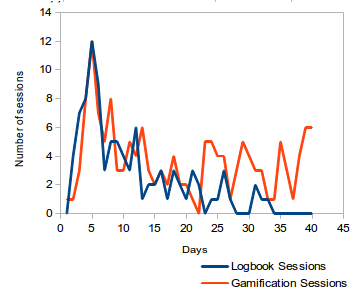
\includegraphics[width=0.5\textwidth]{Figures/scatter_daily_sessions.png}
    \rule{35em}{0.5pt}
  \caption{Average utilization of services and apps by the two groups of participants.}
  \label{figure:usagedailysessions}
\end{figure}\newline
There were two usage comparisons. In the first comparison, I contrasted usage in each day between the Logbook App and Gamified App by computing the daily total number of sessions from all users in a particular experimental condition. There were 41 days in total. Therefore, each day had the total number of sessions in each experimental condition as shown on Figure \ref{figure:usagedailysessions}. After the fourth week there was a decline in usage as the result of the learning effect. The decline was more apparent to users who where switched from gamification to logbook. I used ``\emph{Shapiro-Wilk Normality Test}''\footnote{http://sdittami.altervista.org/shapirotest/ShapiroTest.html} to test for normal distribution between logbook sessions and gamification sessions. The distribution of each of the two independent samples were not normal. An attempt to transform the data using transformation algorithms didn't yield to normal distributions. Therefore, I made a decision to use a non-parametric test called Mann-Whitney U Test. The number of sessions in Gamification condition were significantly higher than in Logbook condition as shown on Table \ref{table:usagedays}.
\begin{table}[h!]
  \begin{center}
    \caption{Daily usage comparison between Logbook and Gamified systems for 41 days}
    \label{table:usagedays}
	\begin{tabular}{|c|c|c|c|c|c|c|}
		\hline
		Groups&N&Rank Average&Sum Ranks&U&Z&P\\
		\hline
   		Logbook sessions&41&33.72&1701.5&\multirow{2}{*}{1159.5}&\multirow{2}{*}{-2.9538}& \multirow{2}{*}{0.00318}\\\cline{1-4} 
   		 		    Gamification sessions&41&49.28& 1701.5&&&\\
\hline
	\end{tabular}
  \end{center}
\end{table}
\newline 
The second comparison entailed contrasting `Logbook'' usage versus ``Gamification'' usage for each pair. I compared usage by counting both the number of days and total number sessions from each pair of users. Since the number of days and total sessions were relative to how many days users were exposed to a particular experimental condition, I divided the number of sessions with total days on which users were exposed to a particular experimental condition to get the ratio of days with respect to the total number of days and number of sessions per day. Therefore, comparison was based on a relative number and not an absolute. For instance, lets say pair one is from a LG group which they had access to a logbook system for 27 days and a gamified system for 14 days. Suppose the number of sessions in Logbook is 50 and the number of sessions in Gamified system is 30 then the relative number of sessions per day spent on logbook is 50 divide by 27 days and the relative number of session spent on  a gamified system is 30 divide by 27. Before comparing the two versions of the system on usage, I had to test if the differences of both the ratio of days and number of sessions per day between the two systems followed a normal distribution in order to identify a proper statistical test to use. The difference between logbook and gamification had a normal distribution in both the ratio of days and number of sessions per day, therefore I conducted a paired t-test. On comparison of usage between a gamified system and logbook system, the former had a higher mean log of ratio of days  and mean log of number of sessions per day compared to the latter without statistical significance.
The results are shown on Table \ref{table:usagewellness1}
\newline 
\begin{table}[h!]

  \begin{center}
    \caption{Usage comparison between Logbook and Gamified systems for 14 pairs of users}
    \label{table:usagewellness1}
	\begin{tabular}{|c|c|c|}
		\hline
		Mean &Logbook App&Gamified App\\
		\hline
		 \multirow{2}{*}{Ratio of days}&M=0.187;SD=0.19&M=0.284 ;SD=0.234\\\cline{2-3} 

		 &\multicolumn{2}{|l|}{t(13)= 1.4714 ; p=0.1650 ; 95\% CI=  -0.239 to 0.0454 } \\
\hline
   		 \multirow{2}{*}{ Number of sessions/day}&M=0.271 ;SD=0.3&M=0.51;SD=0.55\\\cline{2-3} 
		
		 &\multicolumn{2}{|l|}{t(13)=1.5768 ; p= 0.1388 ; 95\% CI= - -0.565 to 0.088} \\
\hline

	\end{tabular}
  \end{center}
\end{table}
\newline  
 
There were four pairs who faced hurdles on utilizing the app and this affected both their motivation and ability to participate or access the system. These pairs are listed on Table \ref{table:usageproblems}.\newline
\begin{table}[h!]
  \begin{center}
    \caption{Pairs with usability/technical problems that hinder their participation}
    \label{table:usageproblems}
	\begin{tabular}{|l|l|l|p{6cm}|}
		\hline
		&Pair&Experimental Sequence&Problem\\
		\hline
		1&Pair A&GL group &App not loading\\
		\hline
		2&Pair B&GL group&Lack of data bundles. \\
		\hline
		3&Pair C & LG group.& Pedometer never transmitted data to the server.\\
		\hline
		4&Pair D & LG group.& Pedometer stopped transmitting data to the server.\\
	\hline
	\end{tabular}
  \end{center}
\end{table}
\newline 
For \textbf{Pair A}, the app failed to load every time their intermediary user tried to use it.What I observed from the house where this pair lived in is that there was a poor Internet signal hence the app was always failing to load most of the time. The second pair (\textbf{Pair B}), data was allocated to the wrong phone number at the beginning of experiments but they never reported on time. These two pairs (Pair A and Pair B) had the lowest usage days which ware 2 and 3 days respectively and they they had used the app only in gamification condition. The last two pairs (\textbf{Pair C} and \textbf{Pair D}) on Table \ref{table:usageproblems} had their pedometers not transmitting steps' data that were important in gamification for advancement of badges, and improvement of both the fish tank and the botanical garden. Pair C's pedometer never transmitted any readings to the server even in logbook condition.  Pair D's pedometer stopped transmitting steps data on the fourth week of running the experiments and this was before this particular user was switched to gamification condition. The two intermediary users from Pair C and Pair D were close friends. Although the pedometer never transmitted data in Pair C,an intermediary user from this pair continued to use the wellness app because of the informal comparison with an intermediary user from Pair D while they were still in logbook condition. The usage in Pair C and Pair D were both eleven days. Their drop out started during gamification condition. Pair C used the app for only three days and Pair D used it for only one day. Since gamification depended on transmission of steps to the server, pedometer problems affected Pair C and Pair D motivations to participate in gamification phase despite their efforts during logbook condition. The learning effect coupled with problems with their pedometers mediated their decrease in usage with the app.  An intermediary user from another pair in "LG" group who happened to live close to the Pair D and Pair C, shared her concerns about the rewards from the gamified app. This was during the endline interviews. This particular intermediary user didn't appreciate her advancement in badges because she admitted that her peers (the two intermediary users from Pair C and Pair D) did more efforts than her but they were not getting anything so she didn't understand why she was ahead of them. She was referring to their usage during logbook condition as they were both using the ``logbook App'' at the same time.  This proves that usability problems played a role to the some extent in demotivating participation in gamification condition  of intermediary users from Pair B and Pair C.\newline
I repeated the above analysis on usage (Table \ref{table:usagewellness1}) without the pairs on Table \ref{table:usageproblems}. Therefore, the new analysis has only ten pairs of users. The differences on ratio of days had a normal distribution shape. A student t test demonstrated that mean ratio of days was significantly higher in the gamified system compared to the logbook system as shown on Table \ref{table:usagewellness2r}. The differences on number of sessions per day didn't have a normal distribution shape. I transformed the data using the natural log equation \ref{equation:log}. The differences between transformed logbook and gamification data followed normal distribution. I performed a paired t test on the transformed data and the results showed that the Log mean of number of sessions per day was significantly higher on gamification condition when compared to logbook condition as shown on Table \ref{table:usagewellness2s}.\newline
\begin{equation}
\label{equation:log}
y=log (x+1)
\end{equation}
\begin{table}[h!]
  \begin{center}
    \caption{Usage on days comparison between Logbook and Gamified systems for 10 pairs of users}
    \label{table:usagewellness2r}
	\begin{tabular}{|c|c|c|}
		\hline
		Mean &Logbook App&Gamified App\\
		\hline
		 \multirow{2}{*}{Ratio of days}&M=0.18;SD=0.18&M=0.35 ;SD=0.25\\\cline{2-3} 

		 &\multicolumn{2}{|l|}{t(9)= 2.3490 ; p=0.0434 ; 95\% CI=  -0.334 to -0.0063} \\
\hline
	\end{tabular}
  \end{center}
\end{table}
\newline  
\begin{table}[h!]
  \begin{center}
    \caption{Usage on sessions comparison between Logbook and Gamified systems for 10 pairs of users}
    \label{table:usagewellness2s}
	\begin{tabular}{|c|c|c|}
		\hline
		Log mean &Logbook App&Gamified App\\
		\hline
		 \multirow{2}{*}{ Number of sessions/day}&M=0.201 ;SD=0.196&M=0.459;SD=0.336\\\cline{2-3} 
		
		 &\multicolumn{2}{|l|}{t(9)= 2.6593 ; p= 0.0261 ; 95\% CI=  -0.477 to -0.039 } \\
\hline
	\end{tabular}
  \end{center}
\end{table}\newline
Baseline data such as demographic information were not statistically sufficient to explain the above usage. However, there was an indication that male intermediaries had higher average number of sessions compared to female intermediaries as shown on Figure \ref{figure:usagegender}.  Also younger intermediaries had higher average number of sessions compared to the old ones as shown on Figure \ref{figure:usageage}.  \newline
\begin{figure}[htbp]
  \centering
    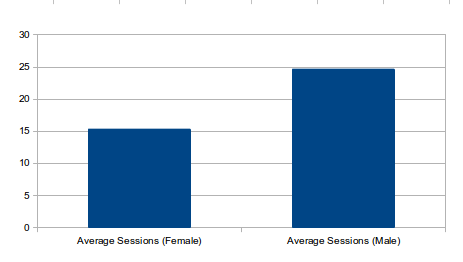
\includegraphics[width=0.5\textwidth]{Figures/session_gender.png}
    \rule{35em}{0.5pt}
  \caption{Average number of sessions between 6 male and 6 female intermediaries.}
  \label{figure:usagegender}
\end{figure}
\begin{figure}[htbp]
  \centering
    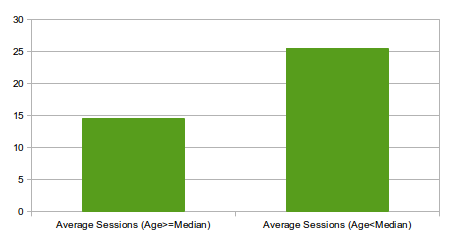
\includegraphics[width=0.5\textwidth]{Figures/session_age.png}
    \rule{35em}{0.5pt}
  \caption{Average number of sessions of 12 intermediaries between age\textgreater=Median(15.5) and age\textless Median(15.5) years.}
  \label{figure:usageage}
\end{figure}
The aforementioned figures were for intermediaries from twelve pairs including Pair C and Pair D on Table \ref{table:usageproblems}. Pair A and Pair B were not considered as they terminated their usage on the first week of experiments pair. Pair B and C were considered as they reported usage up to the fifth week of experiments despite their technical difficulties (4 weeks in logbook and first week of gamification). On the next sub sections, user experiences of both intermediaries and beneficiaries are reported.
\subsection{User Experience of Intermediaries}
User experience was analysed through IMI(Intrinsic Motivation Inventory) questionnaires and interviews. The first step was to examine how baseline intrinsic motivation and  demographic information such as age and gender influence user experience. From Figure \ref{figure:usageage} above, we saw that young intermediaries (age\textless median=15.5 years) appeared to have more number of sessions per day on average, but contrary to this trend is that, at baseline the average perceived enjoyment on helping with cellphone related tasks was higher in intermediaries with age\textgreater=median compared to intermediaries with age\textless median for the 12 intermediary users as shown on Figure \ref{figure:PE_HELP_Age}. 
\begin{figure}[htbp]
  \centering
    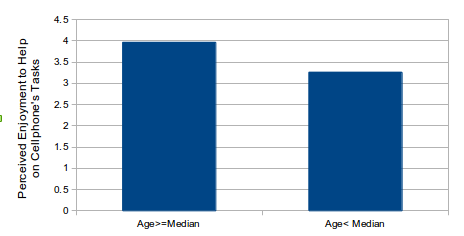
\includegraphics[width=0.5\textwidth]{Figures/PE_HELP_Age.png}
    \rule{35em}{0.5pt}
  \caption{Intermediaries' average perceived enjoyment to help others with cellphone tasks versus age group.}
  \label{figure:PE_HELP_Age}
\end{figure}\newline
I started by comparing the perceived enjoyment to use the family wellness app by age at midline and endline for the 12 intermediary users (excluding users from Pair A and B since they terminated their usage too soon). The purpose of this comparison was to understand why young intermediaries who appeared to be less enjoying on helping with cellphone related tasks, emerged as having more usage sessions than older intermediaries. In this comparison, six intermediary users were below the median age of 15.5 while the remaining six intermediary users were above the median age. More information on these two age groups is provided on Table \ref{table:agregroups}. We can see that both age groups had representatives from both experimental sequences (GL, and LG)  and genders. Figure \ref{figure:PE_Interm_App} shows the averages of perceived enjoyment to use the family wellness app at midline and endline. The averages are higher on the intermediaries with age \textless median for both midline and endline points. \newline
\begin{table}[h!]
  \begin{center}
    \caption{Age groups of intermediary participants}
    \label{table:agregroups}
	\begin{tabular}{|c|L{3.2cm}|L{1cm}|L{2cm}|L{2cm}|L{1.6cm}|L{1.3cm}|}
    		\hline
         &\textbf{Age Groups}&\textbf{Total users}&\textbf{No. of GL sequence}&\textbf{No. of LG sequence}&\textbf{No. of Females}&\textbf{No. of Males}\\
         \hline
         1&Age \textgreater=15.5 years&6&3&3&2&4\\  
\hline
         2&Age \textless15.5 years&6&2&4&4&2\\  
\hline
	\end{tabular}
  \end{center}
\end{table}\newline 
\begin{figure}[htbp]
  \centering
    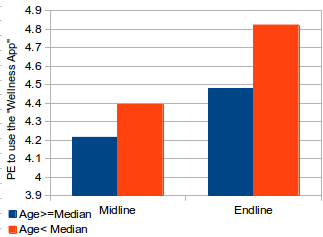
\includegraphics[width=0.5\textwidth]{Figures/PE_Interm_App.png}
    \rule{35em}{0.5pt}
  \caption{Intermediaries' average perceived enjoyment in using the app versus age group.}
  \label{figure:PE_Interm_App}
\end{figure}\newline
There several factors that influence intermediaries to use the app and these are:
\begin{enumerate}
\item{\textbf{Self-monitoring task}}: The task itself of self-monitoring without rewards sparked interests of some intermediary users. This might be as the result of the novelty effect of visualization mechanisms. For instance one intermediary user who happened to be the youngest among all intermediaries reported the highest perceived enjoyment during logbook condition compared to other intermediary users. In addition it seems the phone also had an impact on triggering her interests.
\item{\textbf{Informal comparisons}}: Comparison on steps graphs can be another source motivation. For intermediaries who were close, they did this form of informal comparison. In the absence of gamification, still intermediaries thought that they were competing with other therefore those who were close had face to face interactions of where they did comparison with one another. 
\item{\textbf{Gamification comparison}}: This kind of comparison increased the number of times intermediary user checked the app.
 The ``Gamified App'' was designed in such a way that a pair will earn rewards based on usage and the average number of steps walked by a beneficiary participant who is a member of the pair. The purpose of rewards was to foster users' intrinsic experiences such as competitiveness and a sense of autonomy which are predictors of intrinsic motivation. Rewards depended on four parameters and these were the number of steps walked by a beneficiary user, the number of days the app has been used by an intermediary to either to record meals or to view feedback on meals, points, steps, gardens, etc.
\item{\textbf{Requests from beneficiary users}}:There were times where intermediary users engaged with the app only upon receiving requests from beneficiaries. 
\end{enumerate} 
Intermediaries were interested to fulfil requests from beneficiaries provided an intermediary was interested with the self-monitoring task; steps comparison; or gamification comparison. The trend on average perceived enjoyment in both logbook and gamified conditions appeared to be slightly higher in younger intermediaries compared to older intermediaries as shown on Figure \ref{figure:PE_Interm_App_exp_seq}.
\begin{figure}[htbp]
  \centering
    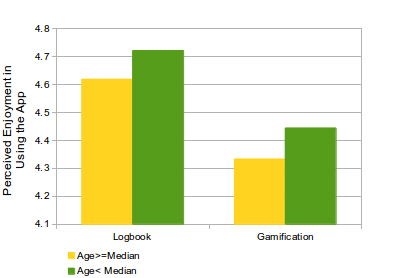
\includegraphics[width=0.5\textwidth]{Figures/PE_Interm_App_exp_seq.png}
    \rule{35em}{0.5pt}
  \caption{Intermediaries' average perceived enjoyment in using the app versus age group (Logbook and Gamification).}
  \label{figure:PE_Interm_App_exp_seq}
\end{figure}\newline

Figures \ref{figure:PE_Interm_App} and \ref{figure:PE_Interm_App_exp_seq}  suggest that the task of helping was more interesting to younger intermediaries due to the existence of the aforementioned motivational affordances. However, not all intermediaries had positive user experience on utilizing gamification, that is why the average perceived enjoyment appears to be lower for both age groups while in gamification condition compared to the logbook condition. If we go back we can see that four pairs had usage problems as mentioned on Table \ref{table:usageproblems}.  From those four pairs, two pairs had severe usability problems and these were pair A and Pair C. Pair B tried to use the app a few times but since they didn't have data bundles usage was terminated immediately, however, the continued to receive SMS feedback throughout the experimental conditions of which some of it was positive as they had managed to attain some badges. User from pair D also appeared to be more interested during gamification even though he terminated usage after his first week on gamification.  We can see that problems in this pair only started on the fourth week of logbook condition (one week before switching to gamification condition), therefore, the  with the pedometer didn't affect much the motivation of the intermediary user from Pair D as he enjoyed the gamification condition despite the fact that he logged in once throughout this experimental condition and the pedometer was not transmitting data to the server. The two users from Pair B and Pair D, had their motivation not affected by usability problems as for Pairs A and C. SMS feedbacks and reminders were sent to all fourteen pairs and this some how engaged users from Pair B and Pair D. During gamification, if a particular pair managed to acquire a new badge, all other pairs were notified through SMS including the pair that had attained a badge. In addition intermediaries were reminded of what has been done and what remains to be done in order to attain higher badges. During logbook condition, intermediaries were notified with SMS of how many steps have been walked by their intermediary so far and they were also reminded that to assist their beneficiaries in monitoring their wellness. Therefore since, usability problems in Pair B and D were not severe as for pairs A and C, and combination of text messages feedbacks, motivation of users in pairs D, and C appeared to be slightly higher in gamification condition compared to logbook condition. From here we can conclude that Pairs A and C motivations during gamification condition were negatively affected by the severe usability problems.\newline 
Gamification condition didn't harm motivation of only users with severe usability problems. There was  a very intriguing phenomenon from two other intermediary users from \textbf{Pair E} and \textbf{Pair F} as mentioned on Table \ref{table:negexprnce}. The two intermediary users had used the app more often in gamification condition  compared to when they were in logbook condition but had reported both lower scores in perceived enjoyment, and perceived competence when in gamified condition compared to when they were in logbook condition. Two of these intermediary users were  in LG and GL groups respectively. I examined the performance of these two users in gamification rewards and discovered that two users never managed to make any progress in attaining a single reward despite their efforts in using the ``Gamified App''. This harmed both their perceived enjoyment and perceived competence to use the "Family Wellness App" while in gamification condition. One of these two intermediary participants sent an SMS to the researcher asking what he was supposed to do in order to advance in badges and he was informed that all the information was specified in their given user manual. In addition, SMS reminders were sent out to all intermediaries to inform them of how far they have gone in achieving rewards and what is remaining in terms of usage and steps in order for them to reach the next badge. Their beneficiary participants were not walking enough steps despite the fact that these intermediaries had put  more efforts in using the App during gamification condition. Badges were earned in combination of both the app usage and average number of steps walked by a beneficiary user. One beneficiary who was working with one of these intermediary users also reported in interviews that there was always a contention with her intermediary when this beneficiary wanted to see what was going in the app as the intermediary was not voluntarily willing to help some of the time.\newline
\begin{table}
  \begin{center}
    \caption{Pairs affected by poor design of gamification}
    \label{table:negexprnce}
	\begin{tabular}{|l|l|l|l|l|L{6cm}|}
		\hline
		&Pair& Experimental Sequence&No. of logbook sessions/day&No. of gamification sessions/day&Challenge\\
		\hline
		1&Pair E&LG group & The beneficiary participant was not walking enough steps hence impacted performance in gamification\\
		\hline
		2&Pair D & LG group.& Same as above.\\
	\hline
	\end{tabular}
  \end{center}
\end{table}
\newline   
Therefore the conclusion was that, the two intermediary users on Table \ref{table:negexprnce}  had a negative experience as the result of failure of our gamification design to match challenges with abilities. i.e. efforts of beneficiaries differed hence challenges should have matched with individual abilities of beneficiaries within pairs. When challenges are too difficult as they don't match users' skills, end users can become demotivated \citep{zhang2008motivational}. As result only eight intermediary users were considered in the main sub scales of intrinsic motivation (autonomy, competence, and enjoyment).\newline
I compared between the logbook and gamification scores from an IMI questionnaire that assessed intrinsic motivation of intermediaries at midline and endline in using the ``The Family Wellness App''. This questionnaire had four sub-scales which where perceived competence, perceived autonomy,perceived enjoyment, and perceived relatedness.  For the reason stated above, I decided to exclude users from  Pair A and C on Table\ref{table:usageproblems} , and Pairs E and F on Table \ref{table:negexprnce}. A total of ten pairs were considered for analysis of on the aforementioned intrinsic motivation sub-scales.\newline
The hypotheses of interest for intermediaries were:
\begin{enumerate}
\item{Hypothesis 1}
\begin{itemize}
\item{H\SB{0}}:There is no difference in perceived competence in using  between a Logbook app and Gamified app
\item{H\SB{A}}:There is a difference in perceived competence in using  between a Logbook app and Gamified app
\end{itemize}
\item{Hypothesis 1}
\begin{itemize}
\item{H\SB{0}}:There is no difference in perceived autonomy in using between a Logbook app and Gamified app
\item{H\SB{A}}:There is a difference in perceived autonomy between a Logbook app and Gamified app
\end{itemize}
\item{Hypothesis 3}
\begin{itemize}
\item{H\SB{0}}:There is no difference in perceived enjoyment in using  between a Logbook app and Gamified app
\item{H\SB{A}}:There is a difference in perceived enjoyment in using between a Logbook app and Gamified app
\end{itemize}
\item{Hypothesis 4}
\begin{itemize}
\item{H\SB{0}}:There is no difference in perceived relatedness in using between a Logbook app and Gamified app
\item{H\SB{A}}:There is a difference in perceived relatedness in using between a Logbook app and Gamified app
\end{itemize}
\end{enumerate}
The results on perceived competence, perceived autonomy,perceived enjoyment, and perceived relatedness of between the ``Logbook App''  and the ``Gamified App'' are shown on Table \ref{table:imiwellnessinterm}. The distribution of the differences of all the scores from the four aforementioned sub-scales, followed a normal distribution hence met a condition for using a paired student t-test.\newline
\begin{table}[h!]
  \begin{center}
    \caption{Comparison of ten intermediaries' scores on sub-scales of competence, autonomy, enjoyment, and relatedness in using the ``Family Wellness App}
    \label{table:imiwellnessinterm}
	\begin{tabular}{|c|c|c|}
		\hline
		Mean &Logbook App&Gamified App\\
		\hline
		 \multirow{2}{*}{Perceived competence}&M=5.23; SD=1.02&M=5.96; SD=0.66\\\cline{2-3} 

		 &\multicolumn{2}{|l|}{t(9)=3.4949; p=0.0068 ; 95\% CI= -1.204 to -0.258} \\
\hline
		 \multirow{2}{*}{Perceived autonomy}&M=3.95; SD=0.86&M=3.96; SD=0.94\\\cline{2-3} 

		 &\multicolumn{2}{|l|}{t(9)= 0.0269; p= 0.9792; 95\% CI= -0.596 to 0.582} \\
\hline
		 \multirow{2}{*}{Perceived enjoyment}&M=4.18; SD=1.11&M=4.75; SD=1.32\\\cline{2-3} 

		 &\multicolumn{2}{|l|}{t(9)= 1.6930;  p=0.1247; ; 95\% CI= -1.343 to 0.193 } \\
\hline
		 \multirow{2}{*}{Perceived relatedness}&M=4.22; SD=0.63&M=4.37; SD=0.9\\\cline{2-3} 
		 &\multicolumn{2}{|l|}{t(9)= 0.7193; p=0.0.4902; 95\% CI= -0.622 to 0.322 } \\
\hline
	\end{tabular}
  \end{center}
\end{table}
\newline
Perceived competence of intermediaries in using the ``Family Wellness App'' was significantly higher in the gamified condition than in the logbook condition in the ten intermediaries that were analysed. Perceived autonomy, perceived enjoyment, and perceived relatedness were all not different between gamification condition and logbook condition. For perceived enjoyment and autonomy, there are cases were the self-monitoring task was interesting enough on itself or when combined with informal comparison of steps among intermediary users. Therefore, there some intermediaries who felt more enjoyment while they were in logbook condition, which is also the same case for perceived autonomy. For perceived relatedness, the app brought users together regardless of an experimental condition especially the ones that already knew each other before.  \newline
\subsection{Beneficiaries' Self-Monitoring of Diet and Activity }
I used the IMI (intrinsic motivation inventory) questionnaire to assess motivation of intermediaries in self-monitoring of Diet. I excluded pairs (A,B, C, and D) from Table \ref{table:usageproblems} problems that led discontinuation of usage. In total only ten out of fourteen beneficiaries had their results included for analysis. We have seen from the sub section (\ref{methodsquestionnaire}) that this questionnaire was administered at baseline, midline and endline.\newline
I compared the IMI score of each participant at baseline, midline, and endline. The IMI score was computed from the average of all scores from sub-scales of perceived competence, perceived autonomy, perceived relatedness, perceived enjoyment, perceived effort,  and perceived usefulness. I  used one way ANOVA with repeated measures to test if there a difference between scores at baseline, midline, and endline. To ensure that we use the correct test, I tested if baseline,midline and endline scores had the same covariance in each case and this helped in deciding of what correction to use on SPSS results among ``Sphericity Assumed'',``Greenhouse-Geisser'', and ``Huynh-Feldt''.\newline 
The results on self-monitoring of diet are shown on Table  \ref{table:imidietbenf}. For self-monitoring of diet, I chose the ``Sphericity Assumed'' since the Mauchly’s test indicated that the assumptionof sphericity was not violated with  $\chi{}$\SP{2}(2)=3.76, p=0.152. Therefore, the results on  ``Self-monitoring of Diet'' shown on Table \ref{table:imidietbenf} is from ``Sphericity Assumed'' output. ANOVA showed that there was a significant difference of average IMI scores on self-monitoring of diet measured at baseline, midline and endline.\newline
\begin{table}[h!]
  \begin{center}
    \caption{Comparison of ten beneficiaries' IMI scores in self-monitoring of diet at baseline, midline and endline}
    \label{table:imidietbenf}
	\begin{tabular}{|L{3cm}|L{2cm}|L{2cm}|L{2cm}|}
		\hline
		Mean IMI Score &Baseline&Midline&Endline\\
		\hline
		 \multirow{3}{*}{Self-monitoring }&M=4.48; SD=1.241; N=10&M=5.07; SD=1.19; N=10;&M=5.55; SD=0.95; N=10\\\cline{2-4} 

		 of Diet&\multicolumn{3}{|l|}{F(2,18)=3.787; p=0.042} \\
\hline	\end{tabular}
  \end{center}
\end{table}\newline
The results on self-monitoring of activity are shown on Table  \ref{table:imiactivitybenf}. For self-monitoring of diet, I chose the ``Sphericity Assumed'' since the Mauchly’s test indicated that the assumptionof sphericity was not violated with  $\chi{}$\SP{2}(2)=3.76, p=0.152. Therefore, the results on  ``Self-monitoring of Diet'' shown on Table \ref{table:imiactivitybenf} is from ``Sphericity Assumed'' output. ANOVA showed that there was a significant difference of average IMI scores on self-monitoring of diet measured at baseline, midline and endline.\newline
\begin{table}[h!]
  \begin{center}
    \caption{Comparison of ten beneficiaries' IMI scores in self-monitoring of activity at baseline, midline and endline}
    \label{table:imiactivitybenf}
	\begin{tabular}{|L{3cm}|L{2cm}|L{2cm}|L{2cm}|}
		\hline
		Mean IMI Score &Baseline&Midline&Endline\\
		\hline
		 \multirow{3}{*}{Self-monitoring }&M=4.48; SD=1.241; N=10&M=5.07; SD=1.19; N=10;&M=5.55; SD=0.95; N=10\\\cline{2-4} 
		 of Diet&\multicolumn{3}{|l|}{F(2,18)=3.787; p=0.042} \\
\hline	\end{tabular}
  \end{center}
\end{table}\newline


As the result of this significant difference, I conducted a student t-test to see if there is a difference on the followings: baseline versus midline, baseline versus endline, and midline versus endline.


\begin{flushright}
\end{flushright}

